\documentclass{article}

\usepackage{fancyhdr}
\usepackage{extramarks}
\usepackage{amsmath}
\usepackage{amsthm}
\usepackage{amsfonts}
\usepackage{tikz}
\usepackage[plain]{algorithm}
\usepackage{algpseudocode}
\usepackage{tikz,pgfplots,multicol}

\usetikzlibrary{automata,positioning}

%
% Basic Document Settings
%

\topmargin=-0.45in
\evensidemargin=0in
\oddsidemargin=0in
\textwidth=6.5in
\textheight=9.0in
\headsep=0.25in

\linespread{1.1}

\pagestyle{fancy}
\lhead{\hmwkAuthorName}
\chead{\hmwkClass\ (\hmwkClassInstructor\ \hmwkClassTime)}
\rhead{\hmwkTitle}
\lfoot{\lastxmark}
\cfoot{\thepage}

\renewcommand\headrulewidth{0.4pt}
\renewcommand\footrulewidth{0.4pt}

\setlength\parindent{0pt}

\setcounter{secnumdepth}{0}
\newcounter{partCounter}
\newcounter{homeworkProblemCounter}
\setcounter{homeworkProblemCounter}{1}
\nobreak\extramarks{Problem \arabic{homeworkProblemCounter}}{}\nobreak{}

%
% Homework Problem Environment
%
% This environment takes an optional argument. When given, it will adjust the
% problem counter. This is useful for when the problems given for your
% assignment aren't sequential. See the last 3 problems of this template for an
% example.
%
\newenvironment{homeworkProblem}[1][-1]{
    \ifnum#1>0
        \setcounter{homeworkProblemCounter}{#1}
    \fi
    \section{Problem \arabic{homeworkProblemCounter}}
    \setcounter{partCounter}{1}
    \enterProblemHeader{homeworkProblemCounter}
}{
    \exitProblemHeader{homeworkProblemCounter}
}

%
% Homework Details
%   - Title
%   - Due date
%   - Class
%   - Section/Time
%   - Instructor
%   - Author
%

\newcommand{\hmwkTitle}{HW \#2}
\newcommand{\hmwkDueDate}{January 26, 2017}
\newcommand{\hmwkClass}{MATH 1300}
\newcommand{\hmwkClassTime}{Section 005}
\newcommand{\hmwkClassInstructor}{Professor Braden Balentine}
\newcommand{\hmwkAuthorName}{\textbf{John Keller}}

%
% Title Page
%

\title{
    \vspace{2in}
    \textmd{\textbf{\hmwkClass:\ \hmwkTitle}}\\
    \normalsize\vspace{0.1in}\small{Due\ on\ \hmwkDueDate\ at 10:00am}\\
    \vspace{0.1in}\large{\textit{\hmwkClassInstructor\ \hmwkClassTime}}
    \vspace{3in}
}

\author{\hmwkAuthorName}
\date{}

\renewcommand{\part}[1]{\textbf{\large Part \Alph{partCounter}}\stepcounter{partCounter}\\}

%
% Various Helper Commands
%

% Useful for algorithms
\newcommand{\alg}[1]{\textsc{\bfseries \footnotesize #1}}

% For derivatives
\newcommand{\deriv}[1]{\frac{\mathrm{d}}{\mathrm{d}x} (#1)}

% For partial derivatives
\newcommand{\pderiv}[2]{\frac{\partial}{\partial #1} (#2)}

% Integral dx
\newcommand{\dx}{\mathrm{d}x}

% Alias for the Solution section header
\newcommand{\solution}{\textbf{\large Solution}}

% Probability commands: Expectation, Variance, Covariance, Bias
\newcommand{\E}{\mathrm{E}}
\newcommand{\Var}{\mathrm{Var}}
\newcommand{\Cov}{\mathrm{Cov}}
\newcommand{\Bias}{\mathrm{Bias}}

\begin{document}

\maketitle

\pagebreak

\section{Graphical Problems}

\begin{enumerate}
\setcounter{enumi}{1}

\item The solid curve in the graph below gives the position $s$ of a car along a straight roadway (measured in meters), as a function of time $t$ (measured in seconds).

\begin{center}\includegraphics[width=6cm]{images/hw2add}\end{center}

	\begin{enumerate}
		\item Find the slope of the dotted line in the graph above. Explain (including units), what this slope represents.
		$$\text{Slope: }\frac{1600}{30}=\frac{160}{3}\approx 53.3 \text{ m/s}$$ In this problem, the slope represents the average meters per second the car travels in the test.
		\item Estimate the instantaneous velocity at $t=15$. Include Units. Draw and label the line you used to estimate this.
		$$\frac{1600-0}{19-11}=\frac{1600}{8}=200\text{ m/s}$$
	\end{enumerate}
	
\item Below is plot of the rainfall accumulation from the 2013 Boulder flood taken from the Foothills Lab Weather Station. The rainfall is measured in millimeters.

\begin{center}\includegraphics[width=0.8\linewidth]{images/boulderfloodgraph}\end{center}

\begin{enumerate}
	\item Use the graph to estimate the average rainfall rate at 04:15 pm (marked as 16:15 on the graph) and 4:15 am the next morning (marked as 05:14 on the graph). Show all work including units. Draw the line that you are finding the slope of. $$\text{4:14pm: }0 \text{ mm of rain}$$
	$$\text{4:15am: }\frac{78-44}{4-1}=11.34 \text{ mm of rain per hour}$$ 
	\item When is it raining hardest? Explain how you know.\\
		It appears that the time with the greatest rainfall is just after midnight (0:15), when the graph has the greatest slope.
	\item Estimate the rainfall rate at 22:15 (including units). Draw the line that you are finding the slope of.\\
		$$\frac{145}{7}\approx 20.72 \text{ mm/s}$$
	\item What does the graph indicate is happening to the rainfall during the hour after 4:15 am?\\
		Because the line has no slope and remains at the same $y$ position, the graph is telling us that the rain stopped at 4:15am.
	\item Explain the precipitous drop between 04:15 and 07:15. \\
		This is when all the rain accumulation vanished in a short period of time, which can also be thought of as a flood.
\end{enumerate}

\end{enumerate}


\section{Section 2.1}

\begin{enumerate}
\setcounter{enumi}{3}
	\item The point $P(0.5,0)$ lies on the curve $y=\cos \pi x$.
	\begin{enumerate}
		\item If $Q$ is the point ($x, \cos \pi x$), use your calculator to find the slope of the secant line $PQ$ (correct to six decimal places) for the following values of $x$:
			\begin{enumerate}
				\item 0 \qquad Slope: $0$
				\item 0.4 \qquad Slope: $4$
				\item 0.49 \qquad Slope: $49$
				\item 0.499 \qquad Slope: $499$
				\item 1 \qquad Slope: $-2$
				\item 0.6 \qquad Slope: $-6$
				\item 0.51 \qquad Slope $-51$
				\item 0.501 \qquad Slope: $-501$
			\end{enumerate}
			\item Using the results of part (a), guess the value of the slope of the tangent line to the curve at $P(0.5,0)$.
			 $$\text{Slope: }500$$
	\end{enumerate}

\end{enumerate}


\section{Section 2.2}

\begin{enumerate}
\setcounter{enumi}{7}
	\item Sketch the graph of the function and use it to determine the values for $a$ for which $\underset{x\rightarrow a}{\lim} f(x)$ exists. 
		
		$$f(x)=\begin{cases} 
      		1+\sin x & \text{if  } x < 0 \\
      		\cos x & \text{if  } 0 \leq x < \pi \\
      		\sin x & \text{if  } x > \pi
   		\end{cases}$$
   		\begin{center}
 		\pgfplotsset{compat=1.6,width=10cm,height=5cm}
		\pgfplotsset{soldot/.style={color=blue,only marks,mark=*}} \pgfplotsset{holdot/.style={color=blue,fill=white,only marks,mark=*}}
 			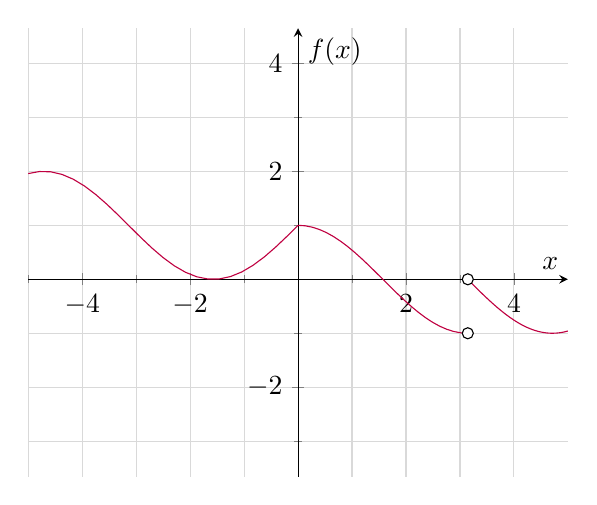
\begin{tikzpicture}
				\begin{axis}[axis lines=middle,xlabel=$x$,ylabel=$f(x)$,axis equal,grid=both,minor tick num=1,grid style={solid, gray!30}]
					\addplot[domain=-5:0,purple] {1+ sin(deg(x))};
					\addplot[domain=0:3.145,purple] {cos(deg(x))};
					\addplot[domain=3.145:5,purple] {sin(deg(x))};
					\addplot+[only marks,mark=*,mark options={scale=1, fill=white},text mark as node=true] coordinates {
					    (3.145,-1)
					    (3.145, 0)};
				\end{axis}
			\end{tikzpicture}
		\end{center}
		$$a = (-\infty,\pi]\cup[\pi,\infty)$$

\setcounter{enumi}{11}
	\item A patient recieves a 150-mg injection of a drug every 4 hours. The graph shows the amount $f(t)$ of the drug in the bloodstream after $t$ hours. Find $$\underset{t \rightarrow 12^{-}}{\text{lim}}} f(t) \qquad \text{and} \qquad \underset{t \rightarrow 12^{+}}{\text{lim}}} f(t)$$ and explain the significance of these one-sided limits.
\begin{center}\includegraphics[width=5cm]{images/22pr8}\end{center}
$$\underset{t \rightarrow 12^{-}}{\text{lim}}} f(t) = 150\qquad
\underset{t \rightarrow 12^{+}}{\text{lim}}} f(t) = 300$$

One-sided limits are almost more crucial than any other kind, as they have real world application. The limits in this problem demonstrate that just before 12, the patient has a very small dosage in their system, but after a booster injection, that amount is doubled to 300mg.

\setcounter{enumi}{14}
	\item Sketch the graph of an example of a function $f$ that satisfies all of the given conditions.
	\begin{itemize}
		\item $\underset{x \rightarrow 3^+}{\text{lim}}} f(x)=4$
		\item $\underset{x \rightarrow 3^-}{\text{lim}}} f(x)=2$
		\item $\underset{x \rightarrow -2}{\text{lim}}} f(x)=2$
		\item $f(3)=3$
		\item $f(-2)=1$
	\end{itemize}
	
\begin{center}
\pgfplotsset{compat=1.6,width=10cm,height=5cm,ymax=5,xmin=-5,xmax=5}
\pgfplotsset{soldot/.style={color=blue,only marks,mark=*}} \pgfplotsset{holdot/.style={color=blue,fill=white,only marks,mark=*}}
	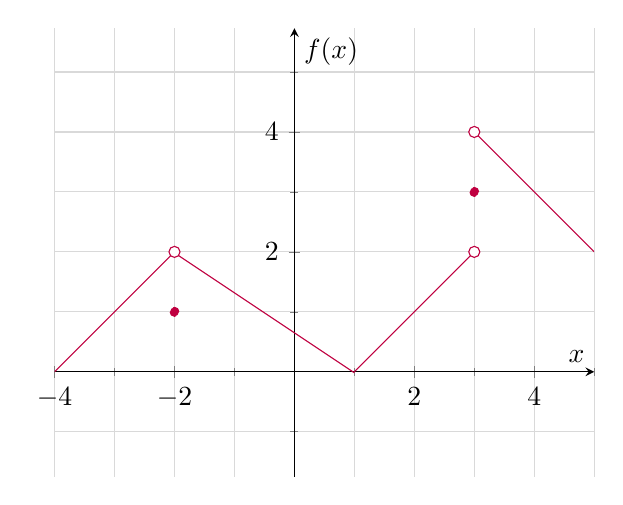
\begin{tikzpicture}
	\begin{axis}[axis lines=middle,xlabel=$x$,ylabel=$f(x)$,axis equal,grid=both,minor tick num=1,grid style={solid, gray!30}]
		\addplot[domain=-4:-2,purple] {x+4};
		\addplot[domain=-2:1,purple] {-(2/3)*x+(0.65)};
		\addplot[domain=1:3,purple] {x-1};
		\addplot[domain=3:5,purple] {-x+7};
		\addplot+[only marks,mark=*,mark options={scale=1, fill=white},text mark as node=true,purple] coordinates {
		    (3,2)
		    (3,4)
		    (-2,2)};
		\addplot+[only marks,mark=*,mark options={scale=0.8, fill=purple},text mark as node=true,purple] coordinates {
		    (3,3)
		    (-2,1)};
	\end{axis}
\end{tikzpicture}
\end{center}

\end{enumerate}

\pagebreak

\section{Challenge Problem}


\begin{itemize}
	\item In 1969, the world record time for the mile was 4:36.8, held by Maria Gommers. 
	\item In 1980, the world record was held by Mary Slaney, with a time of 4:21.7 (data from Wikipedia).
	\item In 1996, the world record was set by Svethlana Masterkova, in a time of 4:12.56
\end{itemize}

Using all the data given, find a shifted exponential model and use it to predict the record in 2050. What is the end-behavior of this model, and what does it represent?

\begin{center}

\pgfplotsset{compat=1.6,width=\linewidth,height=10cm,xmin=60,xmax=160,ymin=220, ymax=300}
\pgfplotsset{soldot/.style={color=blue,only marks,mark=*}} \pgfplotsset{holdot/.style={color=blue,fill=white,only marks,mark=*}}
		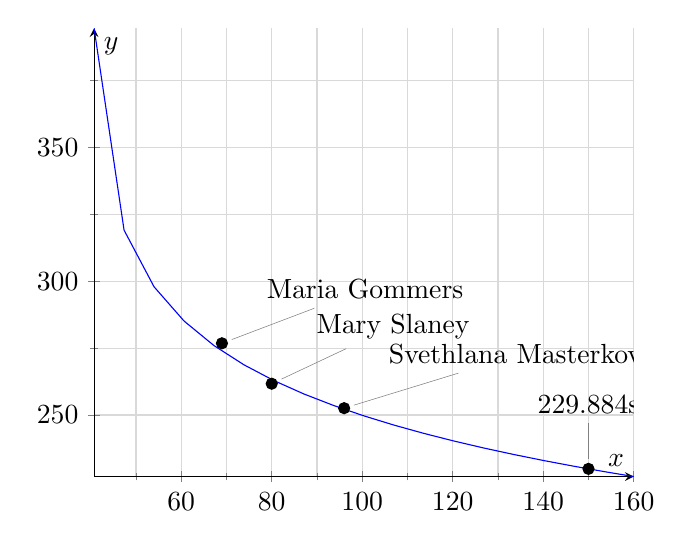
\begin{tikzpicture}
		\begin{axis}[axis lines=middle,xlabel=$x$,ylabel=$y$,grid=both,minor tick num=1,grid style={solid, gray!30}]
			\addplot[mark=*] coordinates {(69,276.8)} node[pin=45:{Maria Gommers}]{};
			\addplot[mark=*] coordinates {(80,261.7)} node[pin=45:{Mary Slaney}]{};
			\addplot[mark=*] coordinates {(96,252.56)} node[pin=45:{Svethlana Masterkova}]{};
			\addplot[domain=1:160,blue] {-33*ln(x-40)+385};
			\addplot[mark=*] coordinates {(150,229.884)} node[pin=90:{229.884s}]{};
		\end{axis}
	\end{tikzpicture}
	$$-33\ln(x-40)+385$$
\end{center}

The end result of this model is that it gets increasingly harder and harder to break the world record, taking nearly 5,500 years to get below 100s. This means that the record will continue to be broken, but less and less often, or by smaller and smaller amounts.

\end{document}